\chapter{Landscape-wide land changes correlate with, but rarely explain local bird diversity change}
%\addcontentsline{toc}{chapter}{Chapter 3}
%\markboth{}{Impacts of past abrupt land change on local biodiversity globally}
\label{C05}

There is an ongoing debate whether biodiversity at local scales is declining and what might drive this change. Land changes are suspected to impact local biodiversity change. However, there is little evidence across spatial and temporal scales and for multiple functional groups of species, thus limiting our understanding of the causes of local biodiversity change. Here we investigate whether landscape-wide land changes, opposed to those at the local scale, are driving local bird diversity change. We link time series of 34 years of breeding bird survey (BBS) data (1984-2017) at 2745 routes across the continental United States of America with remotely-sensed satellite imagery (\textasciitilde30m resolution) from the Landsat missions. Specifically, we assessed for each year what proportion of the landscape surrounding the BBS routes had a land change \textendash\ defined as abrupt shift in magnitude or trend of photosynthetic activity as detected by the Breaks for Additive Seasonal and Trend (BFAST) algorithm \textendash\ and tested whether large proportions of concomitant or preceding landscape-wide land changes explain changes in bird diversity, quantified as either geometric mean of relative abundance (GM) or progressive Bray-Curtis index (pBC). We found that the GM was negatively and the pBC positively correlated with a large proportion of land changes in the wider landscape. Furthermore, the consideration of preceding \textendash\ instead of concomitant \textendash\ landscape-wide land changes explained on average more variation in bird diversity change. Overall, landscape-wide land changes failed to explain most of the variation in local bird diversity change for most BBS routes regardless if bird diversity change is differentiated by functional groups or geographic regions. This study is one of the first studies attempting to link land and biodiversity change. It highlights the influence of preceding and concomitant land change on biodiversity and makes suggestions for promising directions of future research.  

\section{Introduction}
\label{C05_01}

Ongoing human alteration of the Earth surface causes changes in biodiversity across scales \citep{Gibson2011,Murphy2014,Newbold2015}. Globally, about 32\% of all known vertebrate species show decreasing population sizes and range contractions \citep{Ceballos2017,WWF2018} with reported species extinction rates being several times higher than expected naturally \citep{Brooks2002,Pimm2014}. Yet, any change in biodiversity is scale and measure dependent \citep{Sax2003,Chase2013} and, perhaps surprisingly, there is still a debate whether local \textendash\ opposed to global \textendash\ biodiversity is truly changing \citep{Thomas2013,McGill2014}. 

A number of global meta-analyses demonstrated that some biodiversity measures, notably species richness, have not changed at the local scale \citep{Vellend2013,Vellend2017,Dornelas2014}. However, these results have been questioned, particularly on whether the data are spatially and temporally biased \citep{Gonzalez2016} or if sites with and without land change were differentiated \citep{Cardinale2018}. This raises the question whether changes on land can explain changes in local biodiversity measures across space and time. 

Present differences on land influence local biodiversity globally. Previous studies found local biodiversity to be consistently reduced at sites with more intensively used land \citep{Murphy2014,Newbold2015,Alroy2017}, where on average 13.6\% fewer species and 10.7\% fewer individuals were observed compared to undisturbed primary vegetation \citep{Newbold2015}. However, these analyses relied on spatial comparisons of local biodiversity and therefore do not capture temporal biodiversity change. In addition, they ignored the influence of past land changes \citep{Perring2018,Jung2018} and did not consider landscape-wide land changes, which can influence local biodiversity \citep{Tscharntke2012,Turner2015,Miguet2015}. 

Local biodiversity is influenced by the variability of resources, such as food or nesting material, or through ecological processes, such as migration or fear of predation, at the landscape scale \citep{Hanski2000,Chase2003,Turner2015,Fernandez2016}. However these influences are not static and landscapes are constantly changing because of natural and anthropogenic factors \citep{Pickett1985,Manning2009,Turner2015}. Previous studies have shown that landscape-wide land changes may have a lasting influence on local biodiversity through ‘biotic lag’ effects \citep{Metzger2009,Ewers2013}. Yet, most studies focussed on small geographic regions and changes in forest cover \citep{Rittenhouse2010} and did not investigate general impacts of landscape-wide land changes on local biodiversity across spatio-temporal scales. A lack of data on local biodiversity and landscape-wide land change has so far prevented comparative assessments \citep{DePalma2018}.

Increasing availability of satellite imagery enables the assessment of land change at broad spatial and temporal scales \citep{Kennedy2014,Pasquarella2016}. Long-running satellite missions, such as Landsat, provide one of the best sources to monitor land-surface conditions \citep{Kennedy2014,Vogelmann2016,Hermosilla2018,Song2018}. Time series of land-surface conditions, such as photosynthetic activity, can measure intra- and inter-annual vegetation dynamics \citep{Pettorelli2005,Fisher2006} and specific algorithms have been developed to detect land changes as changes in photosynthetic activity \citep{Verbesselt2010,Zhu2017}. Land changes can be differentiated by attributes \citep{Watson2014}, such as abrupt shifts in magnitude, causing an immediate loss or gain of vegetation \citep{DeVries2015b}, or shifts in trend, causing either greening or browning over time \citep{DeJong2013,Muller2014}. These attributes can be robustly quantified at the landscape scale and linked to changes in local biodiversity.

Birds are one of the best surveyed taxonomic groups globally. Local biodiversity change quantified from repeated breeding bird surveys (BBS) has been widely studied \citep{Harrison2014,Pardieck2018}. Previous studies have shown that changes in bird diversity are dependent on the specific biodiversity measure     considered \citep{Schipper2016,Jarzyna2017} and are often non-linear \citep{Gutzwiller2015,Barnagaud2017}. Bird diversity change also varied spatially \citep{Harrison2014,Jarzyna2017} with many birds of particular functional traits, such as migratory or grassland dependent species, declining in developed countries \citep{Fewster2000,Sanderson2006,Stanton2018}. Land changes are most likely a driving factor of these declines \citep{Harrison2014,Harrison2016}, and yet most studies investigated only spatial correlations between remotely-sensed attributes of land change and local bird diversity \citep{Rowhani2008,Goetz2014,Hobi2017}. Notably \cite{Rittenhouse2010} found bird assemblage composition to be altered in landscapes with more “disturbed forests”, which they assessed using remotely-sensed time series. However, to our knowledge, no previous study has investigated whether landscape-wide land changes correlate with and explain changes in local bird diversity.

Consequently, this study hypothesizes that (\textit{i}) changes in local bird diversity are driven by landscape-wide land changes varying by land change attributes, (\textit{ii}) local bird diversity change can best be explained by past land changes, and (\textit{iii}) the explanatory power of landscape-wide land changes on local bird diversity change varies across geographic regions and functional groups of bird species. We combine 34 years (1984–2017) of annual BBS records collected at sites across the continental United States of America with time series of medium-high resolution (nominal \textasciitilde30m) satellite imagery from the Landsat missions. Using Breaks for Additive Seasonal and Trend (BFAST), a generic change detection algorithm, we detect abrupt shifts in magnitude (immediate gain or loss in photosynthetic activity) and trend (greening or browning) of photosynthetic activity in the landscape surrounding each BBS route. Non-linear spatio-temporal models were used to correlate the proportion of changing land in the wider landscape with changes in local bird diversity.


\section{Methods}
\label{C05_02}
\subsection{Bird diversity time-series preparation}
\label{C05_0201}

Time series of local bird count records (1984 – 2017) were obtained from the North American Breeding Bird Survey \citep[BBS, available from \href{https://www.pwrc.usgs.gov/bbs/}{https://www.pwrc.usgs.gov/bbs/},][]{Pardieck2018} dataset. Bird counts were conducted annually during the breeding season (April to August with > 83.3\% sampled in June) along approximately 39.4km long roadside survey routes and usually follow a standard protocol that involves fifty 3min stops at evenly spaced intervals (approximately 0.8km) \citep{Ralph1995}. At each 3min stop, volunteer observers record the number and identity of every bird species seen or heard within approximately 400m distance from the route. For our analyses we only included routes that followed the standard BBS protocol of fifty randomly selected stops (94.4\% of all routes) and had at least ten years of sampling between 1984 and 2017, as many BBS routes were not sampled every year (mean proportion of missing years = 19.7\%). The period from 1984 to 2017 was chosen to align to the availability of satellite data (but see \ref{C05_0202}). We removed routes from the analyses with non-acceptable weather conditions according to BBS standards \citep{Ralph1995} and excluded all nocturnal, crepuscular and aquatic species from the analysis as they are not well sampled by BBS methods \citep{Gutzwiller2015,Jarzyna2017}. All partially identified species (e.g. “sp.”), hybrids and species with unclear taxonomy (\eg  “A x B”) were removed from further analyses. In total, time-series from 2745 routes (out of 5248 in the entire BBS dataset) had suitable data for further analyses.

We calculated two different biodiversity measures commonly applied to BBS data. First, we calculated the geometric mean of relative abundance (GM), which quantifies relative changes in both abundance and evenness \citep{Buckland2011,Buckland2017,Harrison2014}. The GM for the year $y$ is defined as $GM_{y} = \exp(\frac{1}{S} \sum_{i=1}^{S} \log(\frac{ A_{iy}+1 }{A_{iy_0}+1 })$), where $S$ quantifies the total number of species with $i$ being an individual species, $A_{iy}$ the abundance of species $i$ in year $y$. The GM is unaffected by species detectability as it is based on within-species abundance trends, however it cannot be quantified for absent species and is unable to reflect changes in assemblage composition \citep{Buckland2011}. We added a constant (1) to all abundance values before calculating the annual GM to account for the species being absent in some years. The first four years of BBS data (1984 – 1987) were used to define the baseline years $y_{0}$ (calculated from the median number of individuals for each observed species) and to align the analyses with the baseline years used in the land change detection (but see Methods \ref{C05_0203}). Whenever no BBS was conducted in the years between 1984 and 1987 on a given route, we used the first year of available BBS data to define the baseline year $y_0$. Second, as measure of change in assemblage composition, we calculated the progressive Bray-Curtis index \citep[pBC, ][]{Bray1957,Rittenhouse2010} as the difference in composition between a baseline and all following years of sampled bird assemblages \citep{Rittenhouse2010}. The pBC is defined as $ = 1 - \sum_{i=1}^{S} \frac{ |A_{iy} - A_{iy_0}| }{ (A_{iy} + A_{iy_{0}}) } $, where $A_{iy}$ is the abundance of species $i$ in year $y$ and $A_{iy_{0}}$ the estimated abundance in the baseline $y_0$ (defined as for the GM, calculated from the median number of individuals for each observed species).


\subsection{Time series of annual photosynthetic activity at the landscape scale}
\label{C05_0202}

Following previous studies, we define the “landscape” as the 19.7km radius buffer around the centroid of each BBS route because it fully encompasses the majority of BBS routes and approximates the median natal dispersal distance of North American bird species \citep{Sutherland2000,Pidgeon2007,Albright2011}. Grid cells with permanent open water, ice or snow cover were excluded using a land mask derived from the 2011 National Land Cover Database (NLCD) land-cover map at \textasciitilde 30m resolution \citep{Homer2015}. In addition, BBS routes with less than 50\% land area ($N = 18$) within the surrounding landscape were excluded from further analyses, assuming that in those routes breeding birds are less influenced by landscape-wide changes in terrestrial photosynthetic activity.

To quantify land changes in the landscape surrounding each BBS route, we used imagery from the Landsat 4, 5, 7 and 8 satellites (1984 to 2017, \textasciitilde 30m nominal resolution) supplied by the United States Geological Service (USGS) available through Google Earth Engine \citep{Gorelick2017}. All Landsat images were radiometrically \citep{Chander2009} and atmospherically calibrated to surface reflectances \citep{Masek2006}. For each surface reflectance image, we masked out non-land grid cells, including clouds and cloud shadows as identified by the ‘cFMask’ algorithm \citep{Zhu2012}, areas permanently covered with water \citep[> 90\% water occurrence probability in the period 1984 – 2016, ][]{Pekel2016}. A spectral index of photosynthetic activity \citep[the two-band enhanced vegetation index (EVI),][]{Jiang2008} was calculated for each surface reflectance image. We composited all EVI data up to three months before the Summer solstice ($20^th$ of March to $20^th$ June of each year) into a single annual image (1984, 1985, ..., 2017) that retains the greenest (95\% percentile) EVI value. We used three months of EVI data to capture the greening onset in annual vegetation dynamics (Appendix Figure \ref{SI05_01}), a period that can assist in distinguishing between land cover types \citep{Pettorelli2005,Fisher2006,Zhang2006} and that matches the sampling period during which most BBS were conducted (March to June). All data pre-processing and compositing was done using the Google Earth Engine platform \citep{Gorelick2017}.

A lack of clear-sky images in certain years can lead to missing data for parts of the buffered BBS routes. Routes with more than 50\% missing data ($N = 2$) over the period from 1984 to 2017 were excluded from further analyses assuming that the Landsat satellites have missed most land changes (median proportion of missing data = 1.06\% $\pm$ 1.54 median absolute deviation [MAD], Appendix Figure \ref{SI05_02}).

% ---------------- Figure 1 --------------------- %
\begin{figure}[htb]
\centering
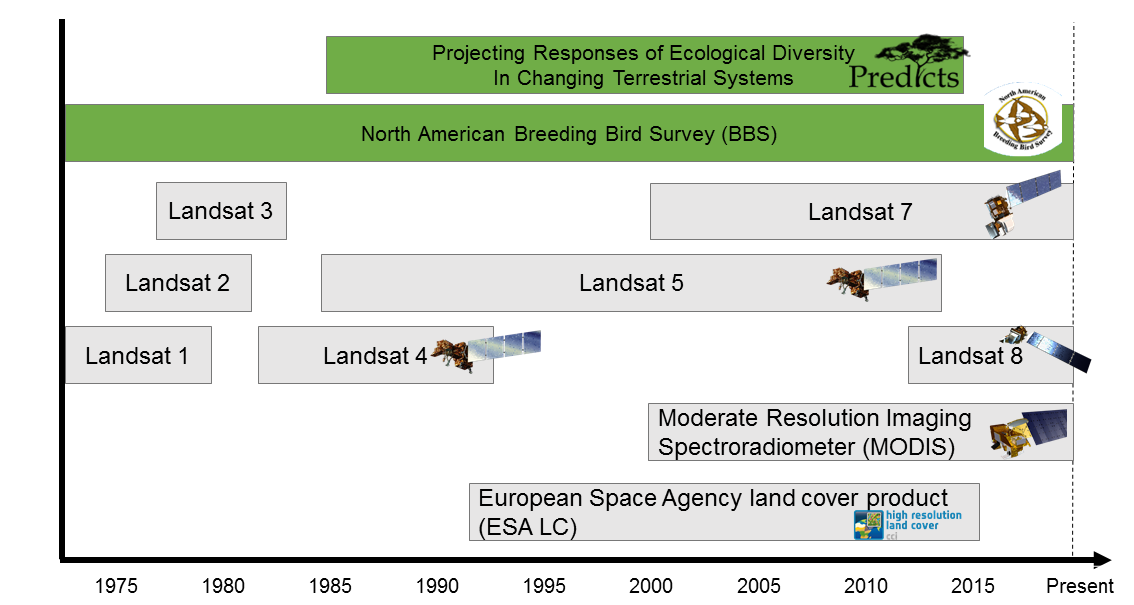
\includegraphics[width=1\textwidth]{chapter5/F01}
\caption{ (\textbf{a}) Schematic how landscape-wide land changes are quantified in a hypothetical BBS route. For each grid cell within the landscape (buffered circle around the BBS route) time series of annual March-June EVI were tested for a single or multiple land changes (see Methods \ref{C05_0203}). If a land change has been detected, we determined the position of all shifts in magnitude (abrupt loss in [“red”] or gain [“blue”]) or trends (greening [“dark green”] or browning [“brown”]) of photosynthetic activity (as measured by the EVI). (\textbf{b}) Changes in local bird diversity (as quantified by the GM and pBC) relative to a baseline year $y_0$ (highlighted in red) for an example BBS route. (\textbf{c}) Summarised proportion of all grid cells within the landscape with either a shift in magnitude or trend in EVI (colours as in \textbf{a}) per year. Map shown in the Albers equal area conic projection (NAD83).}
\label{F05_01}
\end{figure}
% -------------------------------------------- %

\subsection{Detection of landscape-wide land changes as changes in annual photosynthetic activity}
\label{C05_0203}

Landscape-wide land changes were quantified as the proportion of grid cells showing a shift in magnitude or trend of photosynthetic activity (Figure \ref{F05_01}\textbf{a}). Among all algorithms proposed to detect changes in remotely-sensed time series \citep{Zhu2017}, we relied on the generalized fluctuation framework originally developed for econometrics \citep{Bai2003,Zeileis2005}, later adapted for remote sensing as the Breaks for Additive Seasonal and Trend (BFAST) algorithm \citep{Verbesselt2010}. For each annual EVI time series, we tested for single or multiple structural breaks in linear trend using a recursive Moving Sum of Residuals (Rec-MOSUM) test over each four year window period \citep{Zeileis2005}. A statistically significant ($p < 0.05$) structural change test indicates whether at least a single structural break exists, in which case we iteratively fitted segmented linear regression models over the entire time series. The optimal number and position of all structural breaks were detected by minimizing both the Bayesian Information Criterion (BIC) and residual sum of squares (RSS) of the segmented regression models \citep{Zeileis2005,Verbesselt2010}. The framework requires a gap-free time series (“strucchange” package in R, ver. 1.5-1) and similar to previous studies we filled missing data using linear interpolation between adjacent years \citep{Verbesselt2010}.

Per grid cell and year, we differentiated all detected land change events as either abrupt shifts in magnitude or trend (Figure \ref{F05_01}). Shifts in magnitude were quantified using the predicted EVI data (from the segmented linear regression model) before and after the detected change date ($EVI_{After} - EVI_{Before}$) and categorized as either immediate loss or gain in photosynthetic activity in a given year if negative or positive, respectively. For shifts in trend, we assessed for each year whether the linear trend in annual EVI was significantly ($p < 0.05$) increasing (‘greening’), decreasing (‘browning’) or flat (‘stable’). Similarly, for time series with non-significant structural change tests, we fitted simple linear regression models to test whether the overall trend in EVI (across all 34 years) significantly increased or decreased.

For each BBS route and year (Figure \ref{F05_01}\textbf{c}), we summarized the amount of land that had either an abrupt shift in magnitude (loss or gain in EVI) or trend (greening or browning). Because the total land area differed among BBS routes, we calculated proportions relative to the total land area (see Methods \ref{C05_0202}). The change detection algorithm relies on a moving window (four years) and thus no land changes could be detected in the first (1984 - 1987) and last four (2014 - 2017) years of each EVI time series. In case a land change occurred within these years, the algorithm would set the date to the latest, respectively earliest, year possible (\eg 1987 and 2014) causing an inflated number of incorrectly dated land change events at the start and end of each time series. We therefore considered the first four years as ‘baseline’ ($year_0$) and the last four as ‘overhang’ and removed them from further analyses. 

\subsection{Additional predictors and bird trait data}
\label{C05_0204}

At continental scales, bird diversity at BBS routes has been shown to be influenced by a number of environmental variables \citep{Rowhani2008,Goetz2014,Hobi2017,Barnagaud2017}. For a coarse measure of overall vegetation activity \citep{Rowhani2008,Hobi2017}, we calculated the mean EVI across all 34 years of annual Landsat composites per buffered BBS route (see Methods \ref{C05_0202}). Previous studies have shown that the number of bird species varies with elevation \citep{Jarzyna2017} and we extracted the mean     elevation of the buffered BBS route from the global GMTED (\textasciitilde 1km resolution) product \citep{Danielson2011}. Precipitation-driven anomalies have been shown to affect the number and abundance of bird species \citep{Barnagaud2017}. We used the Standardized Precipitation-Evapotranspiration Index (SPEI), which quantifies anomalies relative to the conditions observed in a moving window before a given month \citep{Vicente-Serrano2010,Vicente-Serrano2012}. For each BBS route we extracted the monthly SPEI from SPEIbase \citep[ver. 2.5, \href{http://spei.csic.es}{http://spei.csic.es}, ][]{Vicente-Serrano2010} calculated on a climatology from 1901 to 2015 and over a moving window of three   months from January to March of each year \citep{Vicente-Serrano2010}, thus capturing precipitation anomalies in the winter months.

Similar to previous studies we used four functional trait groups - nesting status, migratory behaviour, habitat guild and body mass - to differentiate all bird species \citep{Schipper2016,Barnagaud2017}. Data on nesting (ground or canopy) and migratory behaviour (resident, short-distance and neotropical migrants) were obtained from \cite{Albright2011}, while data on bird species habitat guilds (\eg woodland, shrubland, grassland and urban birds) were extracted from the USGS website \href{https://www.mbr-pwrc.usgs.gov/bbs/guild/guildlst.html}{https://www.mbr-pwrc.usgs.gov/bbs/guild/guildlst.html}. The mean body mass ($bm$, measured in g) for all bird species was extracted from the Amniote database \citep{Myhrvold2015} and grouped into terciles of all estimates, \eg small, medium and large birds ($bm < 33\%, bm \geq 33\% \& bm < 66\%, bm \geq 66\%$). For species without trait estimates, we filled the missing data with the most common (mode) trait within the same bird genus, provided more than 50\% of all species within that genus had existing body mass estimates or identical categorical trait. For each BBS route and trait group we calculated separate GM estimates, but only for routes with at least 10 years of data and at least 3 different species within a trait group.

